%\chapter{Method}
%\thispagestyle{empty}

\chapter{Framework}
To sparse code images and learn big dictionaries we designed a software
framework called \emph{SPRS}. This section describes the functionality and
decisions made while developing it from idea to implementation.

\section{Signal representation}
\label{sec:signal_representation}
To be able efficiently sparse code images it is necessary to prepare the
image data. As the sparse coding process operates on samples of signal
vectors it is required to transform our 2-D image data in a set of 1-D vectors.
The signal preparation mainly consists of two sub steps. Spatial separation of
the image into blocks and transformation of these into sample vectors.

\paragraph{Spatial separation}
We extract blocks of size $n \times n=m$ from the images. Typically dealing with
block sizes of $n=8,..,20$. The blocks are extracted in a raster either with
overlapping content or disjoint from each other. \prettyref{fig:separation}
illustrates this separation step. 
%How the strategy can effect learning show our experiments.
\begin{figure}[h]
\centering
\subfloat[]{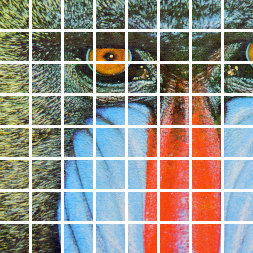
\includegraphics[scale = 0.55]{images/segmentation_new1.png}}
\hspace{5mm}
\subfloat[]{
\includegraphics[scale =
0.50]{images/segmentation2.jpg}}
\hspace{5mm}
\subfloat[]{
\includegraphics[scale =
0.50]{images/segmentation1.jpg}}
\caption[spatial separation]{spatial separation of (a) with (b) and without (c)
overlapping}\label{fig:separation}
\end{figure}

\paragraph{Block transformation} As we are dealing with sets of natural
color images and graphics we primary work with grayscale or three
channel RGB data. 
When dealing with multi-channel data each channel can be coded
separate or as a concatenation of each signal into a single one. Mairal et
al.\cite{mairal08sparse} noticed that the concatenation of the channels leads
to better reconstruction quality. This strategy pays more attention to the fact
that color channels are often highly correlated. But they also notices that both
approaches can lead to color bleeding.  
To address this issue they add a constraint to the sparse coding that pays
attention to correlation of the channels. 
%\Todo{add formula from paper} 
Fortunately Mairal et al. also noticed that this problem vanishes with big
dictionaries and large training sets as present in our experiments. So we use
the concatenation of color channels without a color constraint. 

\begin{figure}[h]
\centering
%\includegraphics[scale = 0.21]{images/channel_concat.pdf}
\label{fig:channel_concat}
\end{figure}
%\cite{mairal08sparse}


\section{Sparse coding step}
When coding a large number of small or medium sized decomposition problems,
which is the case for many samples of small image blocks, some optimizations can
be made on the sparse coding algorithms. 
For the framework we chose to include a batch modified versions of the OMP for
$\ell_0$ regularization and the LARS-Lasso for $\ell_1$ regularization to
address this circumstance. 

\subsection{Batch-OMP}
In 2008 Rubinstein et al.\cite{Rubinstein2008} presented a speed improved
version of the Orthogonal-Matching-Pursuit (\prettyref{sec:omp}) named
\emph{Batch-OMP}. The speed gain is achieved by modifying the OMP in a way to
effectively sparse code multiple signals in parallel. One key element of the
optimizations is the pre-computation of matrix $\mat{G}=\mat{D}^T\mat{D}$ and
$\mat{D}^T\mat{X}$ which can efficiently be reused for each signal. 

Another optimization is the cholesky factorization of $\mat{D}_A^T \mat{D}_A$
(line \ref{alg:OMP_DTD} in \prettyref{alg:omp}). Cholesky factorization is a
process of decomposing a symmetric and positive-definite matrix $\mat{A}$ into
a lower and a upper triangular matrix $\mat{L}$ and $\mat{L}^T$. A triangular
matrix can be inverted more easily. 
$\mat{D}_A^T \mat{D}_A$ is a symmetric positive-definite matrix and can be
cholesky decomposed. Even better, due to the nature of the
algorithm composing $\mat{D}_A$ by adding additional row and columns to it,
$\mat{L}$ can be build up during the computation. This reduces the computational
cost of the algorithm drastically.

\begin{algorithm}[h]
\caption{Parallel coding}
\label{alg:parallel}
\begin{algorithmic}[1]
\REQUIRE $\mat{X} =[\vec{x}_1,...,\vec{x}_k]  \in \mathbb{R}^{m \times k},
\mat{D} =[\vec{d}_1,...,\vec{d}_p] \in
\mathbb{R}^{m\times p}, \epsilon \in \mathbb{R}$
%mat{A} = [\alpha_1,...,\alpha_p] \in \mathbb{R}^{p}
\STATE pre-compute $\mat{G} \gets \mat{D}^T\mat{D}$
\STATE pre-compute $\mat{DtX} \gets \mat{D}^T\mat{X}$
\FOR {$i = 1$ to $k$}
\STATE Compute $\vec{\alpha}_i$ of $\mat{A}$ using \prettyref{alg:lars} or
\prettyref{alg:batchOMP} for all $\vec{x}_i$ in $\mat{X}$
\ENDFOR
\RETURN $\mat{A}$
\end{algorithmic}
\end{algorithm}

\begin{algorithm}[h]
\caption{Batch-OMP}
\label{alg:batchOMP}
\begin{algorithmic}[1]
\REQUIRE $\vec{x} \in \mathbb{R}^{m}, \mat{G}  \in
\mathbb{R}^{m\times m}, \epsilon \in \mathbb{R}$
\STATE $A \gets \emptyset,\vec{\alpha} \gets 0,\vec{r} \gets
\mat{D}^T\vec{x},\vec{\delta}_0 \gets
0, \epsilon_0\gets \vec{x}^T\vec{x},\mat{L}\gets[1],n\gets1$
\WHILE {$ n<L$ \AND $\epsilon_{n-1} > \epsilon $}
\STATE $i \gets \argmax_i\lvert r_i \rvert$
\IF {$n>1$}
\STATE $\vec{w} \gets \mat{L}^{-1}\mat{G}_{A,i}$
\STATE
\begin{align}
\mat{L} \gets \left[
\begin{array}{ccc}
\mat{L} & \vec{0}\\
\vec{w}^T & \sqrt{1-\vec{w}^T\vec{w}}
\end{array}
\right]
\end{align}
\ENDIF
\STATE add variable to active set: $A \gets A \cup \{ i\}$
\STATE $\vec{\alpha}_A \gets (\mat{L}^T)^{-1}\mat{L}^{-1}\vec{\gamma}_A$
\STATE $\vec{\beta} \gets \mat{G}_A\vec{\alpha}_A$
\STATE $\vec{r} \gets \vec{r}-\vec{\beta}$
\STATE $\delta_{n} \gets \vec{\alpha}_A^T\vec{\beta}_A$
\STATE $\epsilon_n \gets \epsilon_{n-1} - \delta_n + \delta_{n-1}$
\STATE $n \gets n+1$
\ENDWHILE
\RETURN $\vec{\alpha}$
\end{algorithmic}
\end{algorithm}

All modifications lead to significant speed increase when coding large sets of
signals. While the maximum number of coefficients $L$ is very small the main
factor of the computation is the multiplication of $\mat{D}$ with a vector.
Batch-OMP reduces the number of those multiplications compared to the ordinary
OMP. Detailed information on the complexity and speed gain can be found in
\cite{Rubinstein2008}. 

% with a complexity of $O(mp)$. 
%This modification reduces the complexity of the OMP from $O\left(L2mp + 2L^2m +
%2L(p+m) + L^3\right)$ to $O\left(2mp + L^2p + 3Lp + L^3\right)$ 
%with pre-computation $\left(mp^2\right)$ as shown in\cite{Rubinstein2008}. 
%more signals than dictionary elements.

\paragraph{LARS-Lasso} is chosen as it one of the fastest $\ell_1$
regularization and it leads to good results for signals of low dimension and
with high correlation of dictionary elements \cite{Mairal2010}. Both conditions
are satisfied when coding small image blocks.

The same pre-computation of the matrix $\mat{D}^T\mat{D}$ and
$\mat{D}^T\mat{X}$ used in the Batch-OMP can also be applied to the LARS-Lasso
algorithm. This also helps to reduce the number of big matrix multiplications
when coding multiple signals in parallel. The framework implements a simple
combination of parallel coding (\prettyref{alg:parallel}) and the
LARS (\prettyref{alg:lars}) presented in \prettyref{sec:lars}.

\section{Learning step}
The majority of learning experiments in literature were made on
samples of sliding blocks from single images or small sets of images.
With extracted samples of $n \ge 100.000$ and sparsness of about 10 non-zero
coefficient. A common strategy when learned dictionaries are only used for
operations on those images. Dictionary atoms learned with this strategy 
have a high correlation to the image content. 
When looking at large sets of images and many different blocks we start to talk
about a different game. Now dictionary atoms tend to capture more
general information of the signals.

For the learning step we use the ODL algorithm from \prettyref{sec:mairal}. As
an online learning algorithm it is able to learn dictionaries from very large
sets of training data $n\ge 10.000.000$.


\subsection{Initialization}
At the start of a training process it is required to initialize the
dictionary with start data. Otherwise the sparse coding step will only find
trivial solutions with all coefficient being zero. Which then will have no
effect in the learning process.

There are two common ways to initialize the dictionary using random data or
selecting random elements from the training data. The framework supports 
both ways of dictionary initialization. 
%\Todo{optional: image}
%can be tested and the quality will be compared.


\subsection{Clustering}
\label{sec:clustering}
One reason not to learn big dictionaries in a single step is the fact that
learning such big dictionaries leads to huge memory consumption and coding time.
To address these problems we investigate strategies to distribute the workload
of the learning step onto multiple clients with a clustering approach similar to
MapReduce. 

One strategy would be to use the mini-batch
modification of the LARS-Lasso (\prettyref{sec:lars}). But rather
than just coding a small batch of signals in one iteration of the training
step (\prettyref{alg:trainDL}) we could code batches in 
a cluster and merge all of them before applying \prettyref{alg:update}. Keeping
the dictionary in each iteration fixed for every batch coding client. The
problem is that this modification is only good at handling mini-batches in a
range of one to thousands samples. Impractical for our desired amount of
millions of samples.

Another strategy is to learn a set of smaller dictionaries $S =
(\mat{D}_1, ..., \mat{D}_k)$ on disjoint training sets. And subsequently merge
the dictionaries $\mat{D}_i$ into a bigger one $\mat{D}_{s}$. 

The merge process starts with an empty dictionary $\mat{D}_{s}$ and
successively adds atoms from the dictionaries of the learning step to the new
dictionary $\mat{D}_{s}$. If the atom can be reconstructed with only a few
atoms of the current dictionary $\mat{D}_{s}$. 
The drawback of this approach is the fact that each atom will be less
correlated with the whole training set. But this will happen anyway as we learn
dictionaries from large sets of possibly very different samples. 

\begin{algorithm}[H]
\caption{Dictionary merging}
\label{alg:merging}
\begin{algorithmic}[1]
\REQUIRE $ S = (\mat{D}_1, ..., \mat{D}_k) \text{ set of dictionaries } \mat{D}
\in \mathbb{R}^{m\times p}$

\STATE $\mat{D}_{new} \gets 0, n \gets 0$
\FOR {$i = 1$ to $k$}
\FOR {$j = 1$ to $p$}
\STATE sparse code: $\vec{d}_j$ of $\mat{D}_i$ with $\mat{D}_{s}$
\IF {$\lVert\mat{D}_{s}\alpha-\vec{d}_j\rVert_2^2 < \epsilon$}
\STATE add $\vec{d}_j$: $\mat{D}_{s}[n] \gets \vec{d}_{j}$
\STATE $n \gets n+1$
\ENDIF
\ENDFOR
\ENDFOR
\RETURN $\mat{D}_s$
\end{algorithmic}
\end{algorithm}



\section{Application to image compression}
\label{sec:compression}
Todays lossy image compression algorithms are primary based on scientific
findings about visual perception reaching far back in the 1970s.
They consist of the following main steps:
% in lossy image compression algorithms:
\begin{itemize}
 \item lossy color space conversion
 \item sub-sampling and spatial separation
 \item transformation of image signals
 \item quantization to reduce the number of non-zero coefficients
 \item lossless entropy encoding of the coefficients 
\end{itemize}

Experiments on sparse coding as a tool for image compression have been done
before\cite{Lewicki1999,Murray2006}. Lewicki compared learned atoms and
generated wavelet atoms. Leading to better results with learned dictionaries
over designed. But entropy encoding was only estimated. 
Real encoding was only applied by Bryt et al.\cite{Bryt2008} in
a very specific algorithm for facial compression. We add quantization and
entropy encoding after the sparse coding step to develop a simple real world
compression algorithm for sparse coding images.


\paragraph{Color conversion and sub-sampling} The human eye is good at sensing
difference in brightness but lacks the ability to exactly differentiate small
changes in color. \emph{Chroma sub-sampling} takes advantage of this human flaw.
First the image gets converted from $RGB$ into $YC_bC_r$ color space, which
describes an image in a brightness ($Y$) and two color components ($C_b$ and
$C_r$). Then the visual more relevant brightness channel will be coded in
the full resolution while the color components can be sub-sampled with
only minor loss in perceptual quality. This procedure is one key element in JPEG
and JPEG 2000 image compression to reduce the number of coefficients for each
color channel. 
But our atoms and samples take advantage of the correlation of the $RGB$ color
channels (\prettyref{sec:signal_representation}). Conversion into $YC_bC_r$ and
splitting the color channels will break the correlation benefit. So we are
skipping this step.  

\paragraph{Spatial separation and signal coding}
The actual coding step of the prepared signals. The signal vectors $\vec{x}_i$
of $\mat{X}$ consist of $n \times n$ non overlapping blocks from the image.
With $n$ in the range $8,...,16$. Similar to the block size and separation
strategy used in JPEG compression. After the signal separation we apply one
of the sparse coding algorithms present in our framework to all blocks. This
step is lossy due to the regularization of sparse coding to chose only a small
number of coefficients. Much less than the dimension of the signal. 

\paragraph{Quantization}  The process of reducing information from a
continuous set of values to a discrete set. In the case of image compression
from double precision to integer values. In our framework the resulting
coefficients from the coding step get divided by a factor and rounded to the
next integer.  

Quantization can either be applied by a fixed factor or by applying different 
factors to each coefficient based on frequency of the basis element.

JPEG quantization uses the fact that the human eye is not good at seeing
differences in high frequency brightness variations. In the development
process of the JPEG algorithm each DCT coefficient was weighted by perceptual
relevance and weights were stored in a quantization matrix. 
This matrix can be applied to the coefficient after the DCT. 
Afterwards each coefficient gets rounded and zero coefficients can be removed.

We adopt the idea of a quantization matrix to our sparse coding approach and
weight our atoms by their frequencies. Learning dictionaries with the
algorithm we present in \prettyref{sec:mairal} leads to a random distribution of
atoms with yet unknown information of their structure and frequency. We analyse
the dictionary atoms with a DFT and sort them by their frequencies.
\prettyref{fig:sorted} illustrates an example of this. Weights are applied
in a simple linear way over the number of elements.

\begin{figure}[h]
\centering
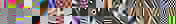
\includegraphics[width = 0.75\textwidth]{images/sorted.png}
\caption{sorted atoms and quantization weights}
\label{fig:sorted}
\end{figure}

\paragraph{Data encoding}
Compression of the remaining coefficients after quantization is the next step
to reduce the amount of data that needs to be stored.

\begin{description}
 \item[Run-length encoding (RLE)] Is the process of encoding repeated data as
blocks of value and corresponding run-length. 
For example the sequence {\bf dddddddbbbddddd} becomes {\bf7d3b5d}.
The main requirement to work well is that the data consists of larger groups of
the same data.
  \item[Huffman coding] An algorithm that analyzes data and 
and replaces elements that occur often in the data set with a shorter symbol.
While 
Leading in a set of symbols and table of . 
% to represent this element and a block of symbols.
\end{description}

We apply something similar to RLE to the sparse matrix. Knowing that the
majority of coefficients in a sparse matrix are zero. They can be coded
as a series of non-zero coefficients and the distances between them.
%We use the fact that in a sparse matrix it is most likely that the entry
%following a coefficient is zero. 
Afterwards the remaining data gets Huffman coded.



%In 1999 Lewicki et al.\cite{Lewicki1999} already made some on comparison 
%the bpp required for encoding of the sparse matrix data. Besides the estimation
%of the compression we also really applied some coding schemes to compare real
%world compression data.
%\cite{Murray2006}


\section{Implementation}
%\subsection*{Software}
The SPRS framework consists of a library (sprscode) for sparse coding image
signals and learning dictionaries, a command line interface (sparsecli) to the
library, miscellaneous scripts for distribution of coding and learning jobs
and a test suite.

The whole sparse coding and training library is written in C++ with
additional use of the OpenCV, Eigen and OpenMP libs. And QMake as the build
system. 

Eigen\footnote{\url{http://eigen.tuxfamily.org/}}
is a template library for fast vector and matrix operations with vector
optimizations and includes some linear algebra algorithms. It is mainly used for
operations on dense and sparse matrices, cholesky factorization and solving of
linear equation systems. All math operations use double precision. 

OpenCV\footnote{\url{http://opencv.willowgarage.com/}} as
in \emph{Open Computer Vision Library} is mainly used for
image read and write operations, image conversion and DCT for the
quantization matrix step. 

OpenMP\footnote{\url{http://www.openmp.org/}} is a preprocessor
based application programming interface (API) for C, C++ and Fortran that
enables the user to distribute code blocks and loops to multiple CPU cores. If
it is applicable OpenMP is used to utilize multi-core CPUs. 


% \Todo{add diagram}
%Split image into sub images, convert sub image to samples from image blocks, 
%train dict with samples or just code samples - save dictionary/image
%Image block size, block selection strategy can be specified.

\paragraph{Coding}
The sparse coding step can be configured to use either the Batch-OMP 
or the LARS-Lasso.
%and 
%set a limitation to the maximum number of coefficients or the
%and set the regularization(\prettyref{eq:l1}) factor $\lambda$.
The Batch-OMP implementation is based on the implementation
of OMPBox by Ron
Rubinstein\footnote{\url{http://www.cs.technion.ac.il/~ronrubin/}} with
technical modifications to fit into our
framework. The LARS-Lasso C++ implementation is based on the Matlab
implementation by Strand\cite{Strand2005} and the original
paper\cite{Efron2004} on the algorithm. With additional optimizations
for coding of multiple signals in parallel. 

\paragraph{Learning}
The dictionary learning step is a straight forward C++ implementation of the
ODL algorithm from \prettyref{sec:mairal}. It is an
implementation of the
basic version of the algorithm with the mini-batch optimization applied.
Batch-OMP and LARS-Lasso can be used for coding part.
Dictionary size and the number training signals for each iteration can be
specified.

\paragraph{Command line interface}
The framework provides a command line interface to the library to unleash its
power. The command line parameters are listed in \prettyref{tab:cli}.
%\lstinputlisting[language=C++,caption=Training]{listings/test.cpp}
\begin{table}[h]
\centering
\begin{tabular}{ |l | l |}
%\hline
%\multicolumn{2}{|c|}{sparsecli}\\
\hline
parameter & description \\
\hline
\verb+--dict <file>+ & save or load dictionary to \emph{file}\\
\verb+--dictSize <n>+ & size \emph{n} of the dictionary  \\
\verb+--train <file>+ & use images listed in \emph{file} as training set\\
\verb+--blockSize <n>+ & size \emph{n} of the image blocks \\
\verb+--winSize <n>+ & size \emph{n} of selection window \\
\verb+--channels <n>+ &number \emph{n} of color channels (1 gray, 3 RGB) \\

\verb+--resume+ & resume an interrupted learning process \\
\verb+--merge <file>+ & merge dictionaries listed in \emph{file}  \\
\verb+--input <file>+ & input \emph{file} for reconstruction \\
\verb+--compress <file>+ & \emph{file} to compress \\
\verb+--uncompress <file>+ & \emph{file} to uncompress \\
\verb+--coeffs <n>+ & maximum number of coefficients \emph{n} \\
\verb+--error <n>+ & reconstruction or merge error \\
\verb+--mode <n>+ & chose \emph{n} either 1 for LARS or 2 for OMP \\
\hline
\end{tabular}
\caption{sparsecli parameters}\label{tab:cli}
\end{table}

\paragraph{Miscellaneous}
Besides the actual coding software some other tools for
additional tasks were used. Several bash and ruby scripts for workload
distribution onto the clients as well as aggregation and evaluation of the
results. 
Also the ImageMagick\footnote{\url{http://www.imagemagick.org/}} toolkit was
used for image conversion into JPEG and JPEG 2000 and for some image comparison
tasks.

%\newpage

